%TC:ignore
In order to build confidence in our system dynamics model and ascertain whether our model is fit for purpose, we conducted tests on model structure and behaviour. These tests are in accordance with \cite{forrester_tests_1980}. Their outputs are shown in this chapter. First, we present the boundaries of the model. Second, we present our findings on the extreme conditions test. Next, we show the results of the sensitivity analysis, and we conclude this chapter by comparing the data of the model to real-world values.

\subsection{Model Boundaries}
A number of variables were considered in conceptualisation of the model, with most excluded from the specification. Explicit definition of variables considered in and out of scope are shown in  Figure \ref{fig:bullseye}.

\begin{figure}[h]
\centering
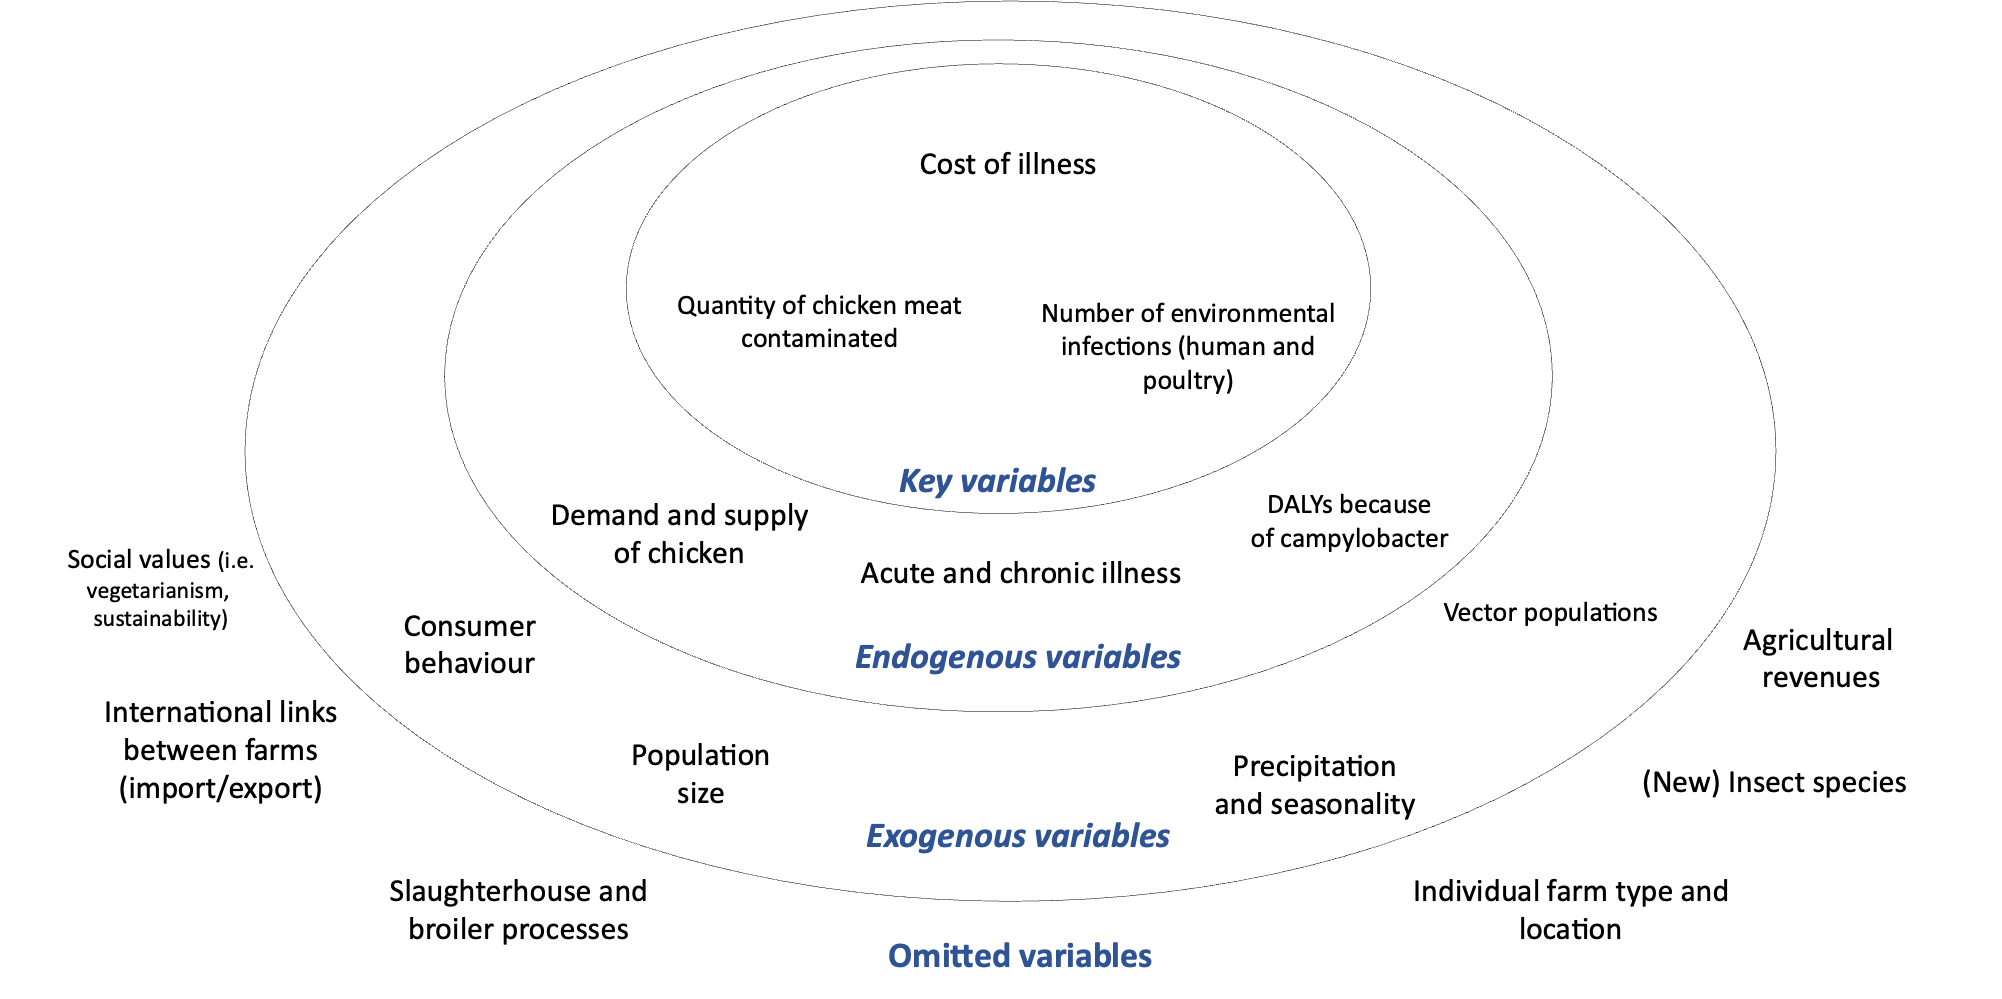
\includegraphics[width=0.90\textwidth]{images/bullseye.png}
\caption{Bullseye diagram for variables considered within model boundaries}
\label{fig:bullseye}
\end{figure}

We included all relevant structures to address the research question. Some structures were left out because they did not fit the aggregation level.

\subsection{Extreme conditions test}
\label{s:extreme_conditions}

To test the structure of the model, we subjected it to extreme conditions to evaluate if the model behaves accordingly. Figures~\ref{fig:temp_fly} to~\ref{fig:reproduction_meat} show the results. The time horizon of these graphs is slightly bigger from the graphs used to show the results. We opted to also show the year the model takes to reach an equilibrium, which results in some interesting behaviour. In other words, we get to see the behaviour of the model in 2020.

As can be seen in Figure~\ref{fig:temp_fly}, the fly population becomes unrealistically high when the temperature gets extremely high. For instance, if throughout the year the Netherlands would have a temperature of 100 \degree c, we would have around 500 times more flies in the Netherlands in summer than in the baseline scenario. This is very unrealistic, as in the real world, those flies would die of the extreme heat. In the graph we show the results when \textit{the temperature increase by 2050} is set to 25 opposed to the 1.5 \degree c of the baseline scenario. The flies are completely unaffected by the harsher environment.

In Figure~\ref{fig:fly_meat}, we show what happens to the KPI \textit{proportion of contaminated meat} once the initial fly population is 0 flies and 1 million flies (1 Mfly). As can be seen, when the population is 0, relatively little meat becomes infected by the environment. However, when it is set to 1 million, we see unusual behaviour before the model reaches homeostasis in 2021. This is impossible behaviour, as a proportion should never be able to become negative or exceed 1. This is because the amount of infectious flies is so big as a result of this initial value, the rate of chicken infection from environment becomes 2.8. In hindsight, the formula should have included a maximum. The vertex of \textit{proportion of contaminated meat} is explained by the fact that there is more demand for chicken meat than is actually available in the stock, therefore both the \textit{contaminated slaughtered chickens} and the\textit{total chickens slaughtered}, which are used to calculate the ratio, are negative. Once equilibrium is reached, the behaviour of the model becomes the same as the behaviour of the baseline: around 50\% of the meats are contaminated in summer, and around 23\% in winter. This is a testament why the first year is out of the time horizon of our research, as it is inaccurate. After this first year the model is still valuable to analyse.

\begin{figure}[h!]
    \centering
    \begin{minipage}{0.45\textwidth}
        \centering
        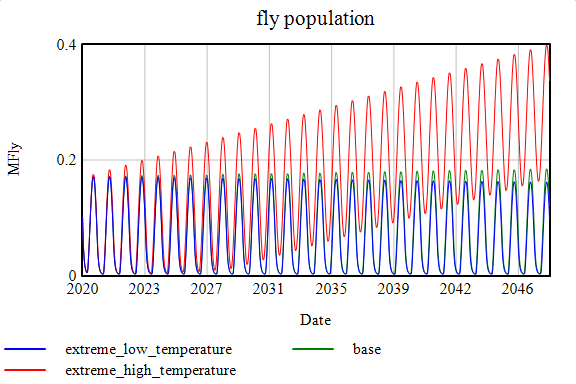
\includegraphics[width=\textwidth]{images/extremes/Temperature_fly_population.png} 
        \caption{Effect of extreme temperature increase values on fly population}
        \label{fig:temp_fly}
    \end{minipage}
    \begin{minipage}{0.45\textwidth}
        \centering
        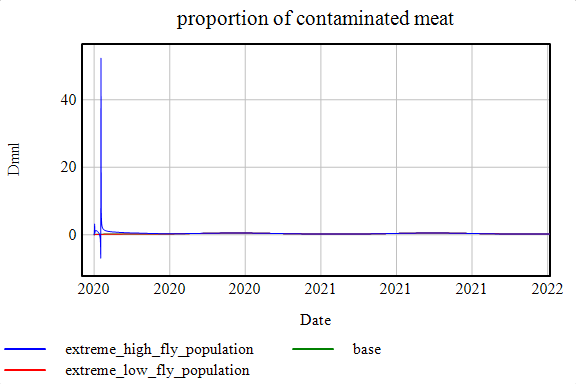
\includegraphics[width=\textwidth]{images/extremes/Fly_population_contaminated_meat.png} 
        \caption{Effect of extreme initial fly population values on proportion of contaminated meat}
        \label{fig:fly_meat}
    \end{minipage}
\end{figure}

We also subjected extremes on the flow \textit{chickens arriving from hatcheries}. The results are shown in Figure~\ref{fig:chicken_meat}. As to be expected, when doubled, the amount of contaminated meat grows massively, this does not propagate to the \textit{Cost of Illness}, as the meats are just stored and the demand has not increased. The meats are just stored (in the model they are just waiting in the stock), whereas halving it actually does decrease the \textit{Cost of Illness}, since the model recognises that the population cannot consume more chicken meat than available, and therefore there is a decreased risk of human infection via food. 

Next, we investigated the \textit{infections per kg of meat consumed}. When the value from the baseline run is halved, we do not see a significance difference in the amount of CPY cases: a decrease of around 3\%, whereas when we multiply this value by twenty, the amount of CPY cases increase with around 170\%. This is more than reasonably can get infected. The model does not account for people who have become immune to \text{Campylobacter}, and therefore the entire population is always at risk of becoming infected. This can be seen in Figure~\ref{fig:infections_cases}

\begin{figure}[h!]
    \centering
    \begin{minipage}{0.45\textwidth}
        \centering
        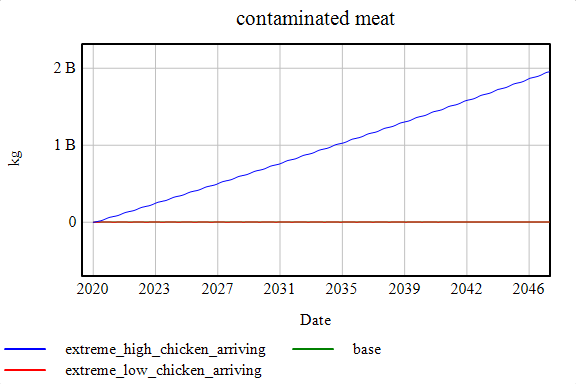
\includegraphics[width=\textwidth]{images/extremes/Chicken_arriving_contaminated_meat.png} 
        \caption{Effect of extreme chicken arriving to hatcheries values on contaminated meat}
        \label{fig:chicken_meat}
    \end{minipage}
    \begin{minipage}{0.45\textwidth}
        \centering
        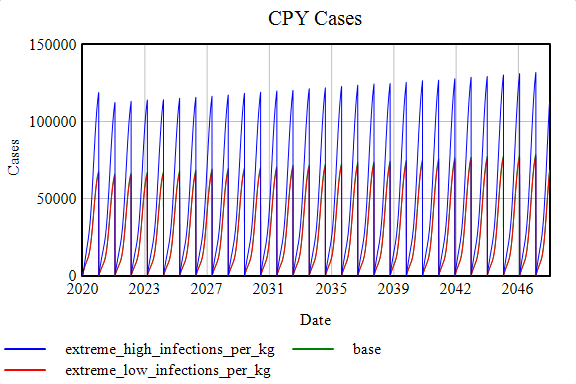
\includegraphics[width=\textwidth]{images/extremes/Infections_per_kg_CPY_cases.png} 
        \caption{Effect of extreme values of infections per kg of meat consumed on Campylobacteriosis cases}
        \label{fig:infections_cases}
    \end{minipage}
\end{figure}

We also took a closer look at the effect of \textit{Base infected flies} on \textit{proportion of infectious flies}. As shown in Figure~\ref{fig:prop_flies}, we found that by setting this value to the extreme 0, the proportion becomes really low.  The only way for flies to get infected in the model is by getting infected by the chickens on the farms. By setting \texit{Base infected flies} to 0.8, the \texit{proportion of infectious flies} variable becomes an impossible ratio (over 1). This is due to the formula used to calculate the proportion, which adds the base infectious flies to the amount of flies infected by chickens. 

Next, we investigated the effect of \textit{base chicken exposure rate} on the KPI \textit{contaminated meat}. The results of the extremes we subjected the model to can be seen in Figure~\ref{fig:exposure_meat}. The value used in the baseline is 0.1, and by setting it to 0, we see a decrease in \textit{proportion of contaminated meat} of around 20\% in both summer and winter. It nearly reaches a proportion of 0 in winter. When it is set to 0.8, the proportion is, once again, unreal. More than 100\% of the meat is contaminated in the summer. This is because there are more \textit{contaminated slaughtered chickens} than \textit{total chickens slaughtered}, which is also something that is impossible in real life. It is caused by the fact that we neglected including a floor function the \textit{CPY-negative chickens} stock. There simply are not enough CPY-negative chickens, and it therefore turns negative. Because of this, a negative amount of chickens are slaughtered with and without cross-contamination, which decreases the \textit{total chickens slaughtered}.

\begin{figure}[h!]
    \centering
    \begin{minipage}{0.45\textwidth}
        \centering
        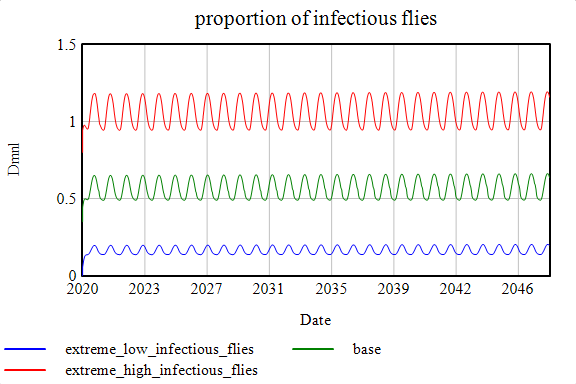
\includegraphics[width=\textwidth]{images/extremes/base_infectious_flies_proportion_flies.png} 
        \caption{Effect of extreme base infectious flies values on proportion of infected flies}
        \label{fig:prop_flies}
    \end{minipage}
    \begin{minipage}{0.45\textwidth}
        \centering
        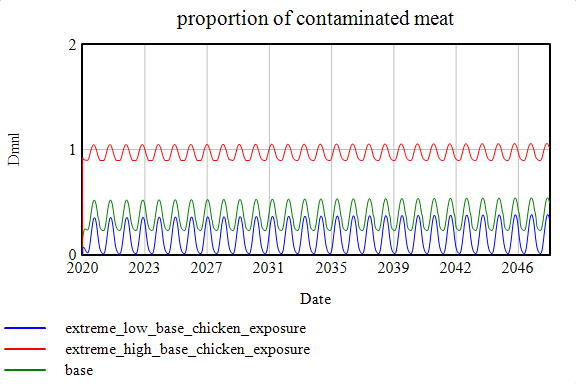
\includegraphics[width=\textwidth]{images/extremes/Base_chicken_exposure_contaminated_meat.png} 
        \caption{Effect of extreme base chicken exposure rates on proportion of contaminated meat}
        \label{fig:exposure_meat}
    \end{minipage}
\end{figure}

Finally, we explored the extremes of \textit{CPY reproduction in chickens}. When it is set to the extreme 4, the model reports a proportion of contaminated meat greater than 1, which is an unreasonable proportion. The explanation for this behaviour is similar to the explanation of the previous extreme conditions test: there are more contaminated chickens slaughtered than total chickens slaughtered.This is because the flow \textit{slaughtering without cross-contamination} is always negative, and therefore decreases the \textit{total chickens slaughtered}. The behaviour of this flow is explained by the value of \texit{rate of cross contamination}, which is around 2.4 in the summer. The reason for this high rate can be directly traced back to \texit{CPY reproduction in chickens}, which is used as a multiplyer in \texit{rate of cross contamination}. At the other extreme, we see a decrease in \textit{contaminated meat consumption}, with the most significant difference in summer (a decrease of 40\% opposed to 25\% in winter). This is simply because there is significant less contaminated meat to consume (about 1 million kg less).

\begin{figure}[h!]
    \centering
    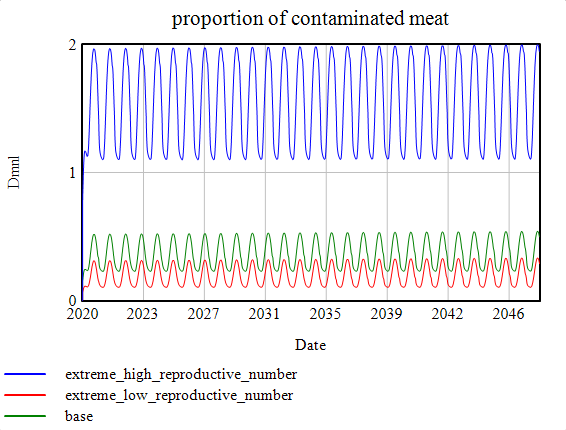
\includegraphics[width=0.45\textwidth]{images/extremes/CPY_reproduction_contaminated_meat.png} 
    \caption{Effect of extreme CPY reproduction on proportion of contaminated meat}
    \label{fig:reproduction_meat}
\end{figure}

%The extreme high value of temperature increase evidences a problem in the model, as fly reproduction is unreasonably high since extreme temperatures are likely to create a harsher environment for them as well. For the extreme high values of initial fly population and base infectious flies, the model reports a proportion of contaminated meat that is greater than the total amount of meat, which should not be possible. A similar thing happens with base infections flies and base chicken exposure rate, which can cause more infectious flies than there are total flies. When chicken arriving from hatcheries are decreased (and thus made lower than the demand), the model can handle the situation because it does not allow for consumption of more chicken that are available, but when instead it is raised, the excess supply is never dumped, creating an issue of accumulating meat indefinitely which is not realistic. Lastly, when infections per kg of meat consumed are raised 20 times its original value, it can bring issues of too many people being infected, since our model does not account for immunity of population, all population is indefinitely susceptible which becomes a problem when infection numbers are very big.

\subsection{Sensitivity Analyses}
To realise the model, we resorted to assumptions, as certain data was unavailable. We were interested in knowing how sensitive the model was to changes in these parameters. We wanted to assess the impact of the parametric changes under all 3 types of scenarios, individually, and combined.

\subsubsection{Univariate Sensitivity Analysis}
With univariate sensitivity analysis only one parameter was varied at a time, while the other parameters of the system remained constant. We wanted to test all submodels of our system and therefore varied the following parameters: \textit{projected population by 2050}, \textit{temperature increase by 2050}, \textit{temperature switch},  and \textit{rate of symptomatic case modifier}. The first parameter determines population growth, the second parameter determines the maximum temperature of the next 30 years, the third parameter determines how temperature is expected to increase, and the laast parameter how many people will actually show symptoms when infected with \textit{Campylobacter}.

\paragraph{Population growth}
Based on population projections \parencite{nidi_nidi_2020} we ran the sensitivity analysis and got the results in figures \ref{fig:pop_coi}, \ref{fig:pop_meat}, \ref{fig:pop_chicken}, and \ref{fig:pop_human}. Because a population increase also increases demand for chicken, generating a reaction across the model than can be appreciated in the increased contaminated chicken meat stock as well. Because more people get infected in total and present symptoms, the cost of illness also increases.

\begin{figure}[h!]
    \centering
    \begin{minipage}{0.45\textwidth}
        \centering
        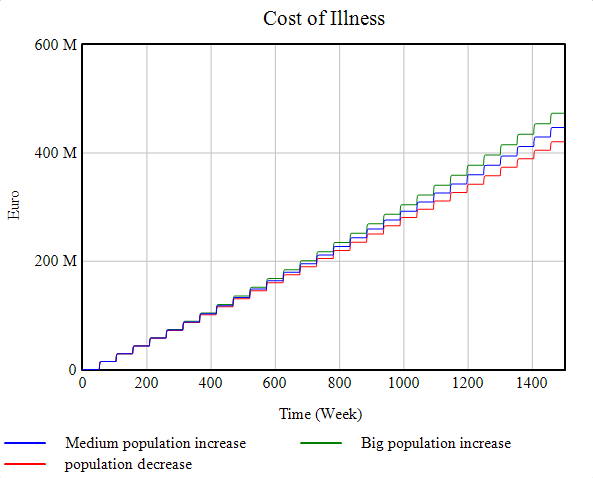
\includegraphics[width=1\textwidth]{images/sensitivity/Population COI.png} % first figure itself
        \caption{Cost of Illness in the different population scenarios}
        \label{fig:pop_coi}
    \end{minipage}\hfill
    \begin{minipage}{0.45\textwidth}
        \centering
        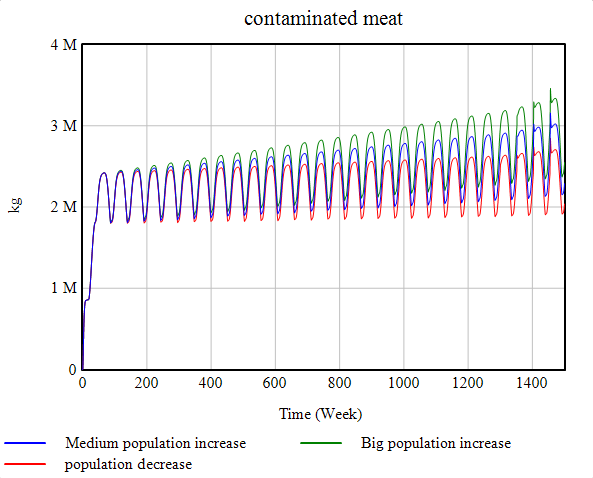
\includegraphics[width=1\textwidth]{images/sensitivity/Population contaminated meat.png} % second figure itself
        \caption{Contaminated chicken meat in the different population scenarios}
        \label{fig:pop_meat}
    \end{minipage}
\end{figure}

\begin{figure}[h!]
    \centering
    \begin{minipage}{0.45\textwidth}
        \centering
        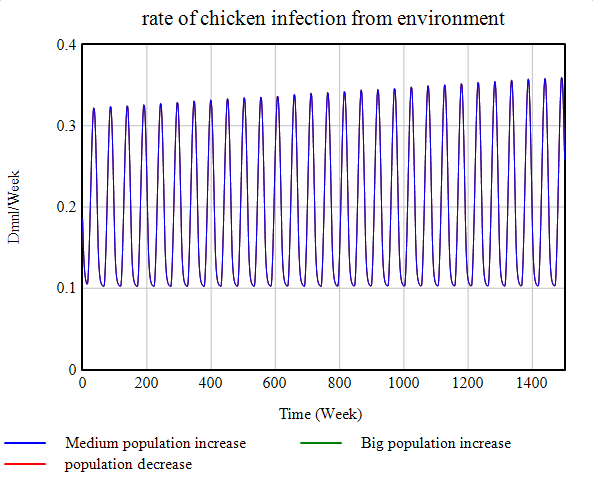
\includegraphics[width=1\textwidth]{images/sensitivity/Population chicken infection.png} 
        \caption{Chicken infections from environment in the different population scenarios}
        \label{fig:pop_chicken}
    \end{minipage}\hfill
    \begin{minipage}{0.45\textwidth}
        \centering
        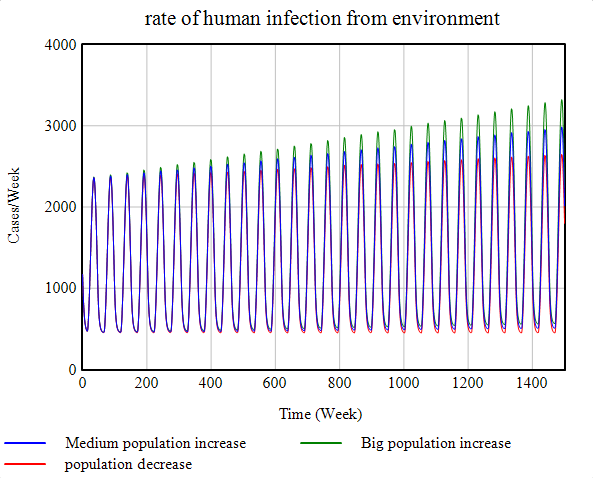
\includegraphics[width=1\textwidth]{images/sensitivity/Population human infection.png}
        \caption{Human infections from environment in the different population scenarios}
        \label{fig:pop_human}
    \end{minipage}
\end{figure}

\paragraph{Average temperature increase}

Based on climate change projections \parencite{knmi_knmi_2015} we ran the sensitivity analysis and got the results in figures \ref{fig:temp_coi}, \ref{fig:temp_meat}, \ref{fig:temp_chicken}, and \ref{fig:temp_human}. Temperature increasing aids in the development of disease vectors, which has a direct impact on human infections, besides also affecting indirectly through the food borne route of transmission. This results in increased cost of illness proportional to the increase in temperature over the years.

\begin{figure}[h!]
    \centering
    \begin{minipage}{0.45\textwidth}
        \centering
        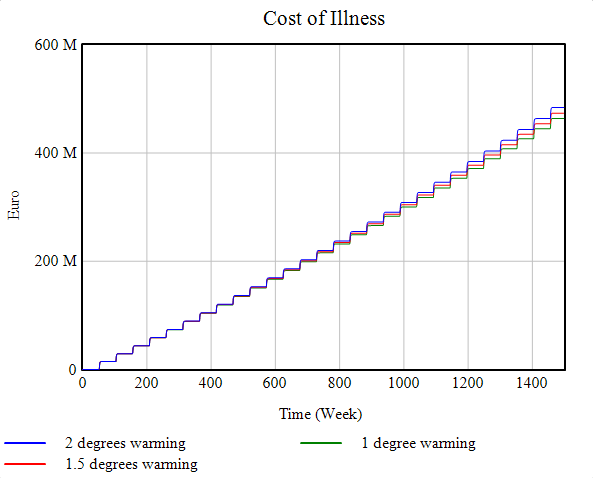
\includegraphics[width=1\textwidth]{images/sensitivity/Temperature projection COI.png} % first figure itself
        \caption{Cost of Illness in the different temperature increase scenarios}
        \label{fig:temp_coi}
    \end{minipage}\hfill
    \begin{minipage}{0.45\textwidth}
        \centering
        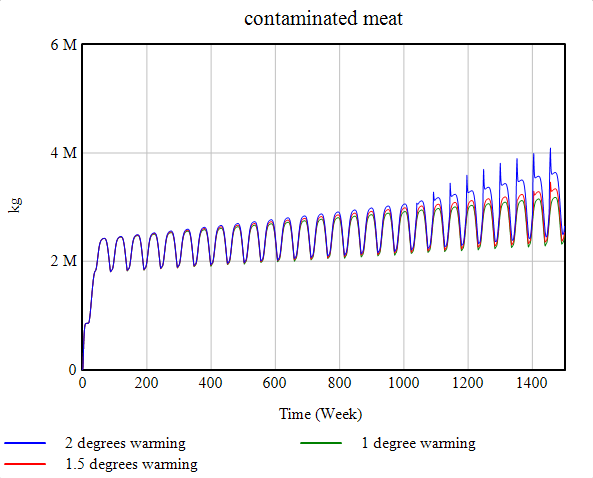
\includegraphics[width=1\textwidth]{images/sensitivity/Temperature projection contaminated meat.png} % second figure itself
        \caption{Contaminated chicken meat in the different temperature increase scenarios}
        \label{fig:temp_meat}
    \end{minipage}
\end{figure}

\begin{figure}[h!]
    \centering
    \begin{minipage}{0.45\textwidth}
        \centering
        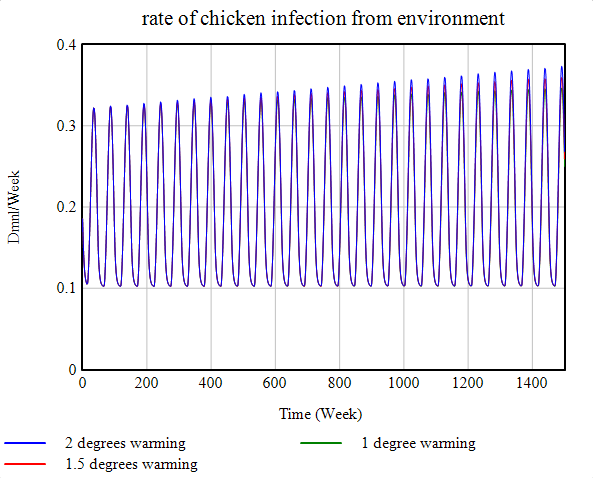
\includegraphics[width=1\textwidth]{images/sensitivity/Temperature projection chicken infection.png} 
        \caption{Chicken infections from environment in the different temperature increase scenarios}
        \label{fig:temp_chicken}
    \end{minipage}\hfill
    \begin{minipage}{0.45\textwidth}
        \centering
        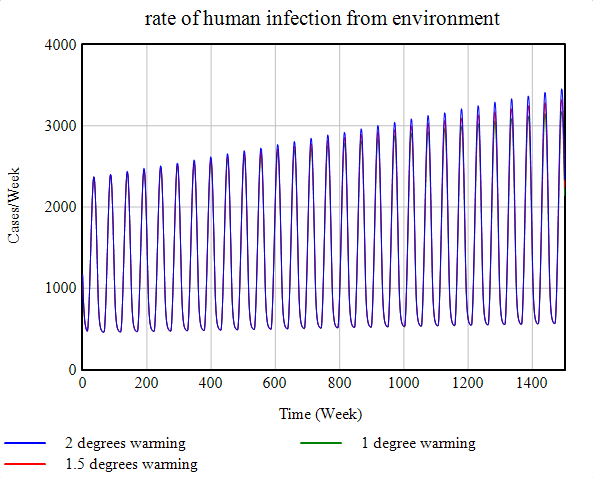
\includegraphics[width=1\textwidth]{images/sensitivity/Temperature projection human infection.png}
        \caption{Human infections from environment in the different temperature increase scenarios}
        \label{fig:temp_human}
    \end{minipage}
\end{figure}

\paragraph{Seasonal temperature increase}

There is uncertainty in how the temperature might increase in the future. It seems that the increase is not uniform throughout the year, but that instead summers might warm up faster than winters. We modelled this uncertainty and compared the scenarios. The seasonal variation in temperature increase leads to longer warmer periods compared to cold periods, which also affects disease vector propagation and has an impact in infections and subsequently in the cost of illness. This can be appreciated in figures. \ref{fig:season_coi}, \ref{fig:season_meat}, \ref{fig:season_chicken}, and \ref{fig:season_human}.

\begin{figure}[h!]
    \centering
    \begin{minipage}{0.45\textwidth}
        \centering
        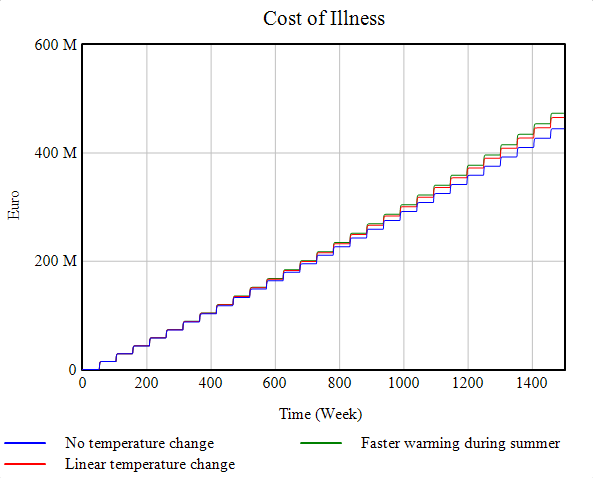
\includegraphics[width=1\textwidth]{images/sensitivity/Seasonal temperature COI.png} % first figure itself
        \caption{Cost of Illness in the different temperature seasonality scenarios}
        \label{fig:season_coi}
    \end{minipage}\hfill
    \begin{minipage}{0.45\textwidth}
        \centering
        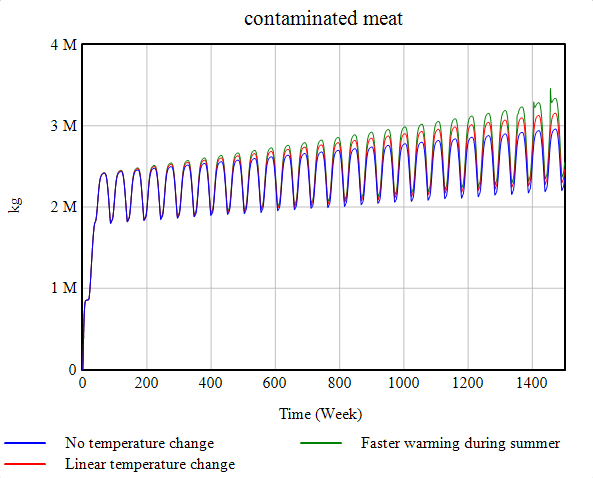
\includegraphics[width=1\textwidth]{images/sensitivity/Seasonal temperature contaminated meat.png} % second figure itself
        \caption{Contaminated chicken meat in the different temperature seasonality scenarios}
        \label{fig:season_meat}
    \end{minipage}
\end{figure}

\begin{figure}[h!]
    \centering
    \begin{minipage}{0.45\textwidth}
        \centering
        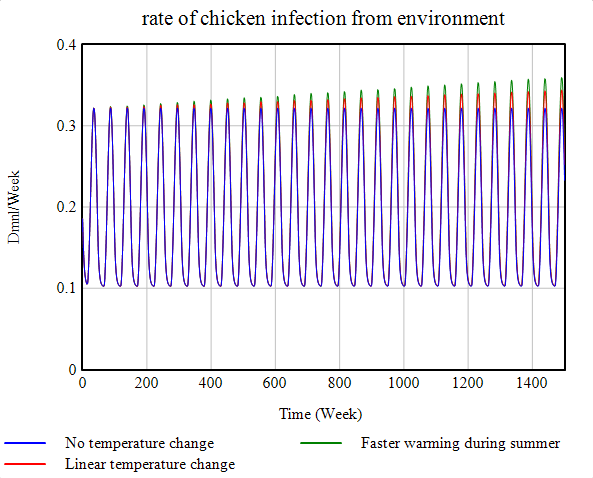
\includegraphics[width=1\textwidth]{images/sensitivity/Seasonal temperature chicken infection.png}
        \caption{Chicken infections from environment in the different temperature seasonality scenarios}
        \label{fig:season_chicken}
    \end{minipage}
    \begin{minipage}{0.45\textwidth}
        \centering
        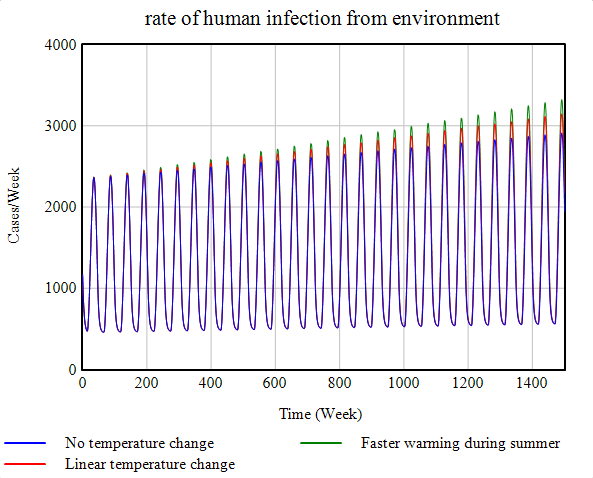
\includegraphics[width=1\textwidth]{images/sensitivity/Seasonal temperature human infection.png}
        \caption{Human infections from environment in the different temperature seasonality scenarios}
        \label{fig:season_human}
    \end{minipage}
\end{figure}

\paragraph{Rate of symptomatic infections} %multiple?

On figure \ref{fig:symptom_COI} we can see the result of rate of symptomatic infections changing, which is a behaviour that has been observed recently \parencite{medema_assessment_1996}. This only bring changes to the cost of illness, as infections remain the same across the model, but the severity of the disease requires more treatment.

\begin{figure}[h!]
    \centering
    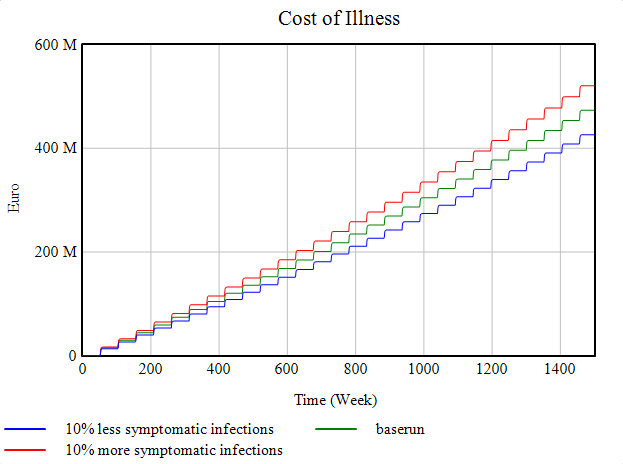
\includegraphics[width=0.45\textwidth]{images/sensitivity/Symptomatic COI.png} 
    \caption{Cost of illness in the different symptomatic infection scenarios}
    \label{fig:symptom_COI}
\end{figure}

\subsubsection{Multivariate Sensitivity Analysis}

We ran multivariate analysis to account for the compounded effect of different uncertainties, and the results can be found in Figures \ref{fig:multi_coi}, \ref{fig:multi_meat}, \ref{fig:multi_chicken}, and \ref{fig:multi_human}. We employed VenSim's built-in Sensitivity feature and let it run 200 simulations. We assigned certain parameters a maximum of 110\% of their original value, and a minimum of 90\% of their original value. The parameters we subjected to this were: \textit{temperature increase by 2050}, \textit{projected population by 2050}, \textit{temperature switch}, \textit{rate of symptomatic cases modifier}, \textit{COI modifier}. The \textit{COI modifier} was a variable we built in purely for the Multivariate Sensitivity Analysis, as it is uncertain whether the costs for treating the chronic conditions changes overtime. The observed change is mostly regarding numerical sensitivity, but we can see that the contaminated chicken meat can overshoot at times, which is the result of people refusing to eat meat as a result of increased infections, but the chicken were already in the production cycle so there was excess production.

\begin{figure}[h!]
    \centering
    \begin{minipage}{0.45\textwidth}
        \centering
        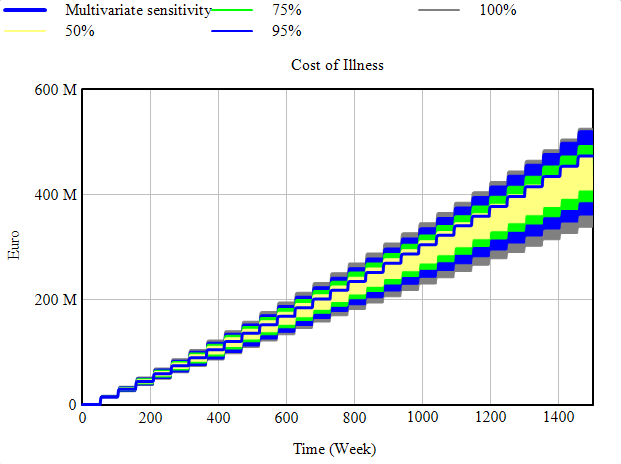
\includegraphics[width=1\textwidth]{images/sensitivity/Multivariate COI.png} % first figure itself
        \caption{Cost of Illness in the multivariate analysis}
        \label{fig:multi_coi}
    \end{minipage}\hfill
    \begin{minipage}{0.45\textwidth}
        \centering
        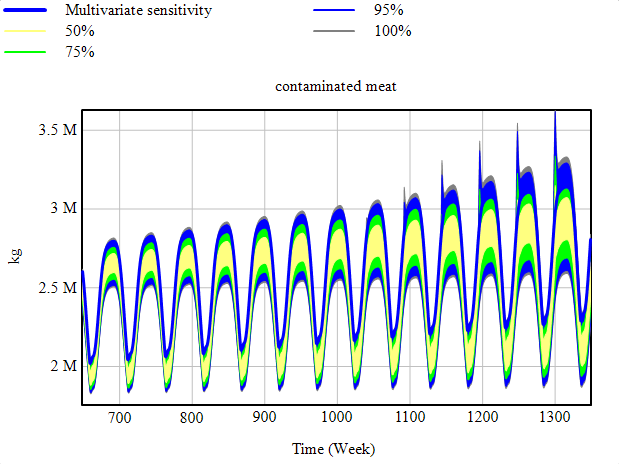
\includegraphics[width=1\textwidth]{images/sensitivity/Multivariate contaminated meat.png} % second figure itself
        \caption{Contaminated chicken meat in the multivariate analysis}
        \label{fig:multi_meat}
    \end{minipage}
\end{figure}

\begin{figure}[h!]
    \centering
    \begin{minipage}{0.45\textwidth}
        \centering
        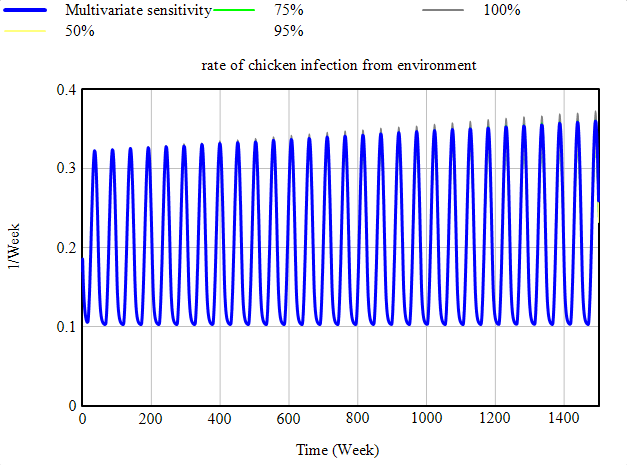
\includegraphics[width=1\textwidth]{images/sensitivity/Multivariate chicken infection.png} 
        \caption{Chicken infections from environment in the multivariate analysis}
        \label{fig:multi_chicken}
    \end{minipage}\hfill
    \begin{minipage}{0.45\textwidth}
        \centering
        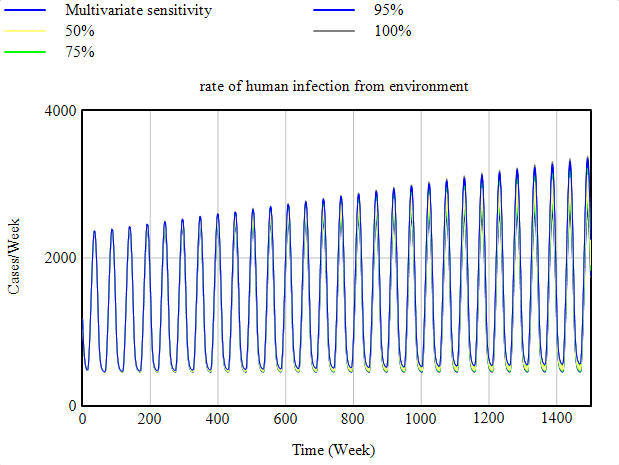
\includegraphics[width=1\textwidth]{images/sensitivity/Multivariate human infection.png}
        \caption{Human infections from environment in the multivariate analysis}
        \label{fig:multi_human}
    \end{minipage}
\end{figure}


\subsection{Comparison to real world data}

\textcite{vlaanderen_staat_2019} estimated there were around 71.000 cases of Campylobacteriosis in the Netherlands in 2018, 67.000 in 2017 and 79.000 in 2016. We plotted the amount of cases produced by our model against the average of these three values. The results can be seen in Figure~\ref{fig:val_human_cases}. We can see the stock in our model is a good reflection of the real world. 

\textcite{nepluvi_rapportage_2019} monstered broiler chickens weekly in 2018, and found $41,9$-$58.1\%$ of broiler chickens were tested positive for \textit{Campylobacter}. This concerns chickens from slaughterhouses. As can be seen in Figure~\ref{fig:val_chickens}, our base model has similar values for each year.

In the Netherlands the (unsanitary) preparation and/or consumption of chicken were attributed to $20$-$30\%$ of infections in 2018. However, around $50$-$80\%$ of cases can be attributed to \textit{Campylobacter} strains associated with poultry \parencite{cuperus_surveillance_2020, nepluvi_rapportage_2019}. Therefore, it is safe to assume that there are multiple transmission routes. We assume the biggest transmission routes can be found in the environment. In the base model, around 5.77\% of the infections stem from the preparation and/or consumption of chicken. This can be seen in Figure~\ref{fig:val_sources}. It may be the case that the environment plays a bigger role than we previously assumed, after all, it is easier to trace back the cause to undercooked meat than to a wild bird.

Numbers on the average amount of chicken meat consumption per Dutch person differ, but they are between 0.22 and 0.47 kg of chicken meat per week~\parencite{schotman_europese_2018, waveningen_university__research_we_2020}. In our model this fluctuates between 0.153 and 0.203 so there is a slight discrepancy.

We also validated our DALYs and Cost of Illness against the data points from \parencite{mangen_campylobacteriosis_2007}. Note that these values are from 2007. As can be seen in Figure~\ref{fig:val_dalys} our model determines higher DALYs than given in the literature. This may indicate that there are more chronic diseases that can be traced back to \textit{Campylobacter} than is currently happening in the real world. Perhaps the specialists are overlooking the bacterium as a cause, or they are simply unable to pinpoint the cause.

In Figure~\ref{fig:val_coi} it can be seen that the Cost of Illness calculated by the model is lower than \citeauthor{mangen_campylobacteriosis_2007}'s values. This is probably due to the fact that we only look at 3 chronic conditions and the acute conditions. 

It is estimated there are around 17 million species of \textit{Diptera} per person \parencite{gorman_trillions_2017}. We are only interested in \textit{Musca domestica}. It is unknown what their numbers are in the Netherlands, and we are unable to estimate. However, it has been guessed that the population of Houseflies will increase by 244\% by 2080 \parencite{mcalister_secret_2017}. In The amount of flies in our model after 1 year is 20.000 of which 7.700 are infectious (TIME STEP = 0.0625). This is probably not a proper reflection of the real world, but one can assume that it is only 7.700 flies that have directly caused a disease in humans and/or chickens.

The model also includes an Infection risk from birds (2.5e-05). There are about 1.3 million birds in the Netherlands \parencite{noauthor_miljoenen_2019}. There was no literature on the risk from birds, so we assumed a somewhat safe value. We doubt \textit{Campylobacter} will ever be exterminated due to the presence of these environmental factors, even if we are somehow able to keep our farms, slaughterhouses and stores free from \textit{Campylobacter}.



\begin{figure*}[!h]
    \centering
    \begin{minipage}{0.45\textwidth}
        \centering
        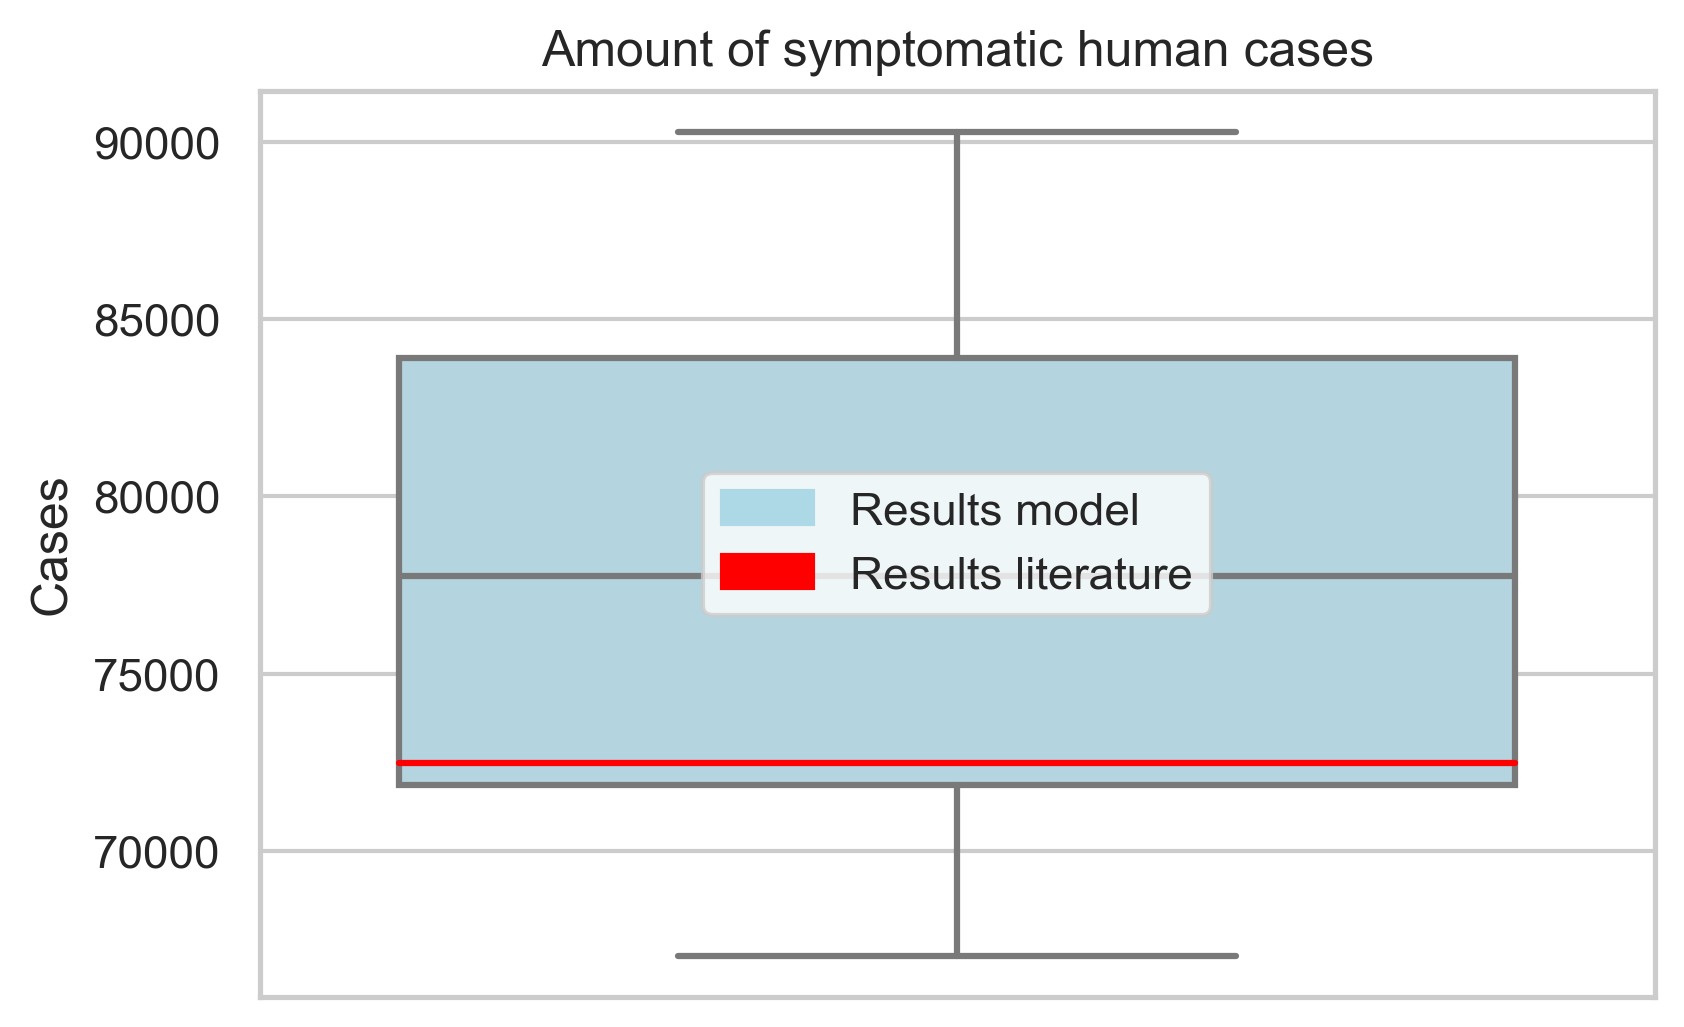
\includegraphics[width=0.9\textwidth]{notebooks/human_cases2.png} % first figure itself
        \caption{Validation of human cases}
        \label{fig:val_human_cases}
    \end{minipage}\hfill
    \begin{minipage}{0.45\textwidth}
        \centering
        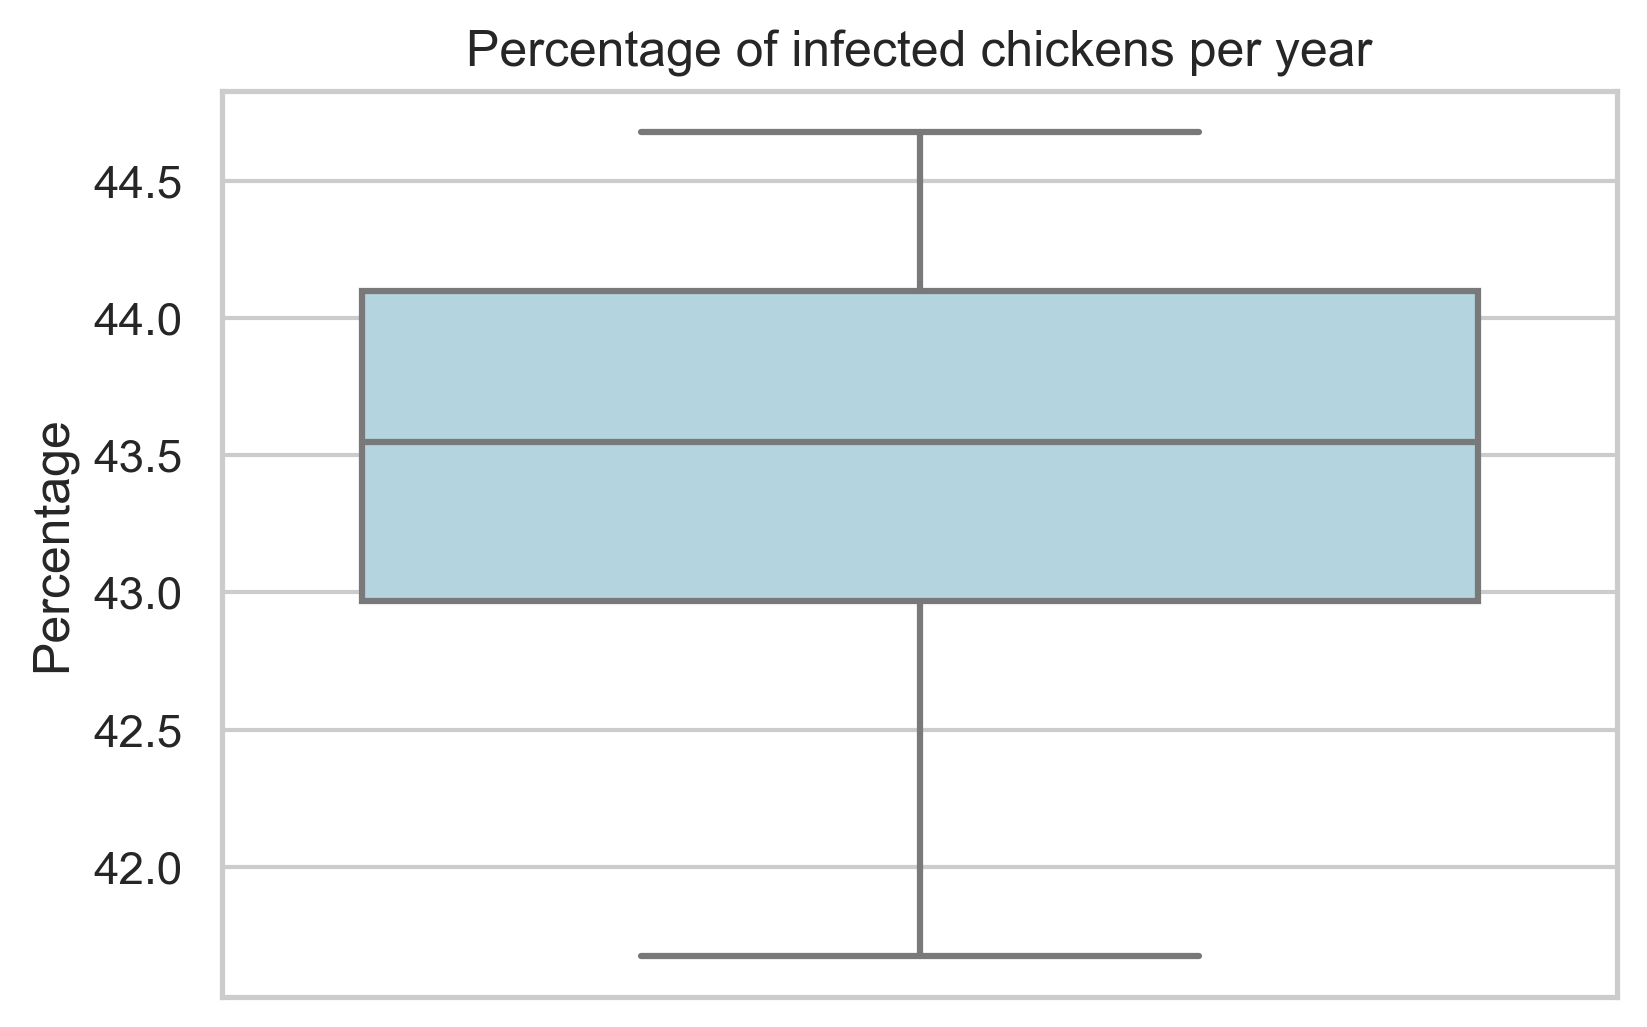
\includegraphics[width=0.9\textwidth]{notebooks/chickens2.png} % second figure itself
        \caption{Validation of proportion infected chickens}
	    \label{fig:val_chickens}
    \end{minipage}
\end{figure*}

\begin{figure*}[!h]
	\centering
	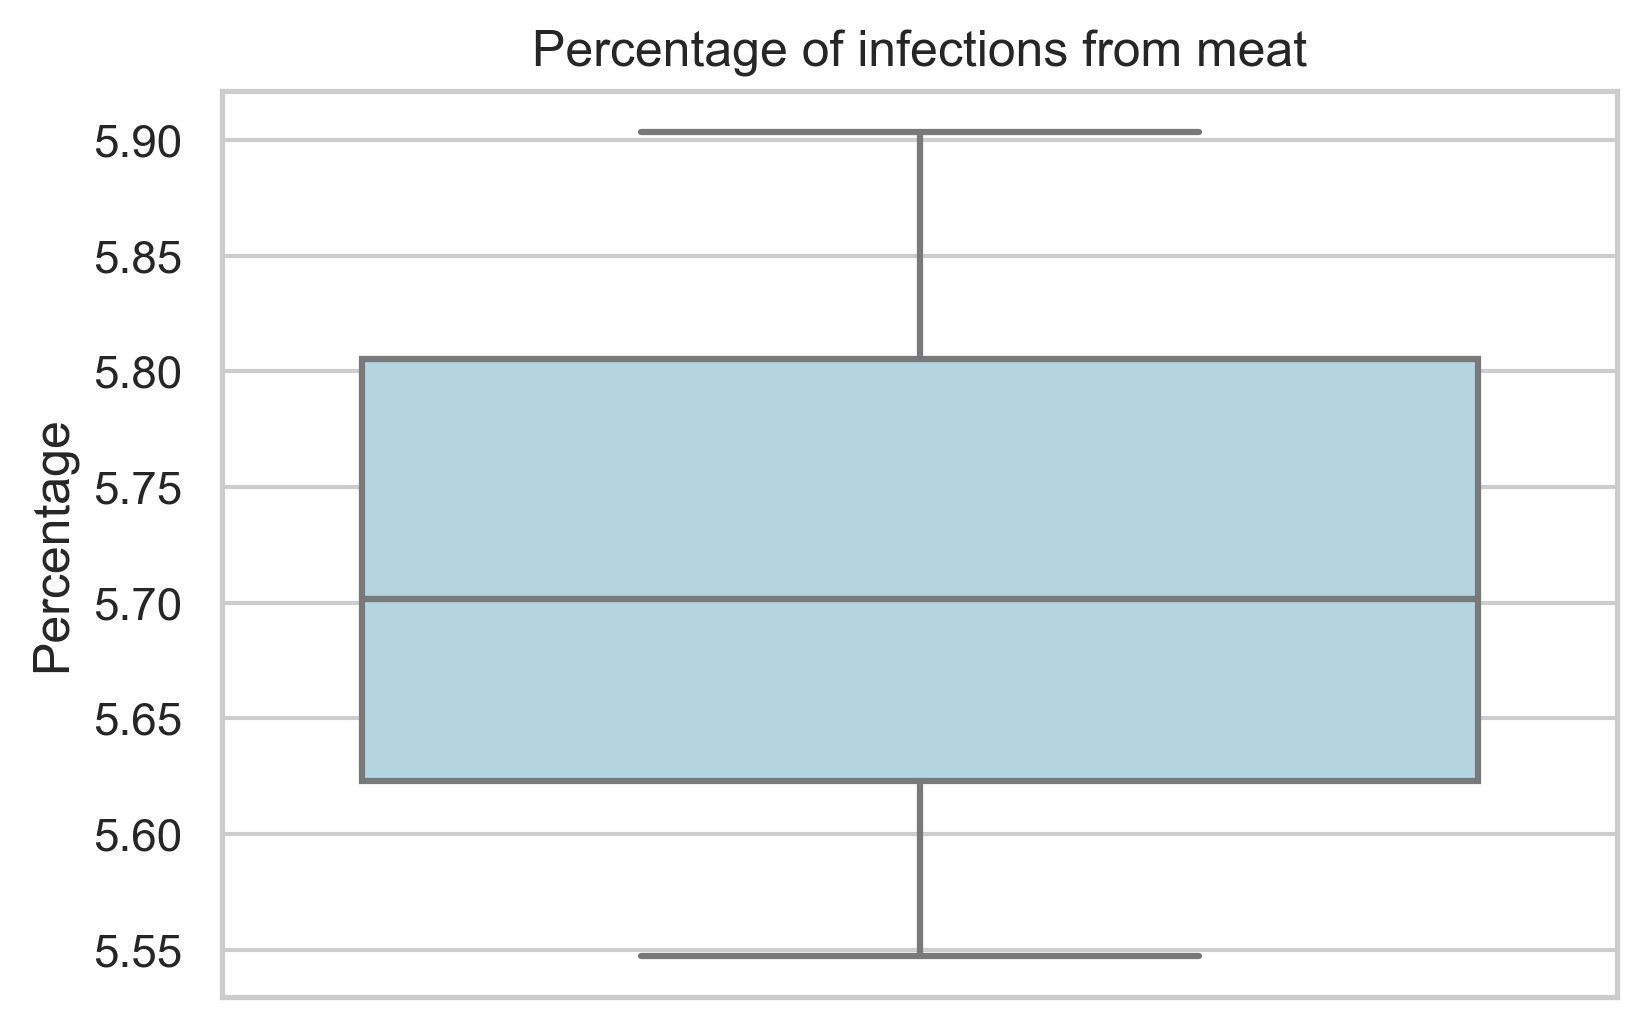
\includegraphics[width=0.5\textwidth]{notebooks/source2.png}
	\caption{Validation of sources of Campylobacteriosis}
	\label{fig:val_sources}
\end{figure*}

\begin{figure*}[!h]
    \centering
    \begin{minipage}{0.45\textwidth}
        \centering
        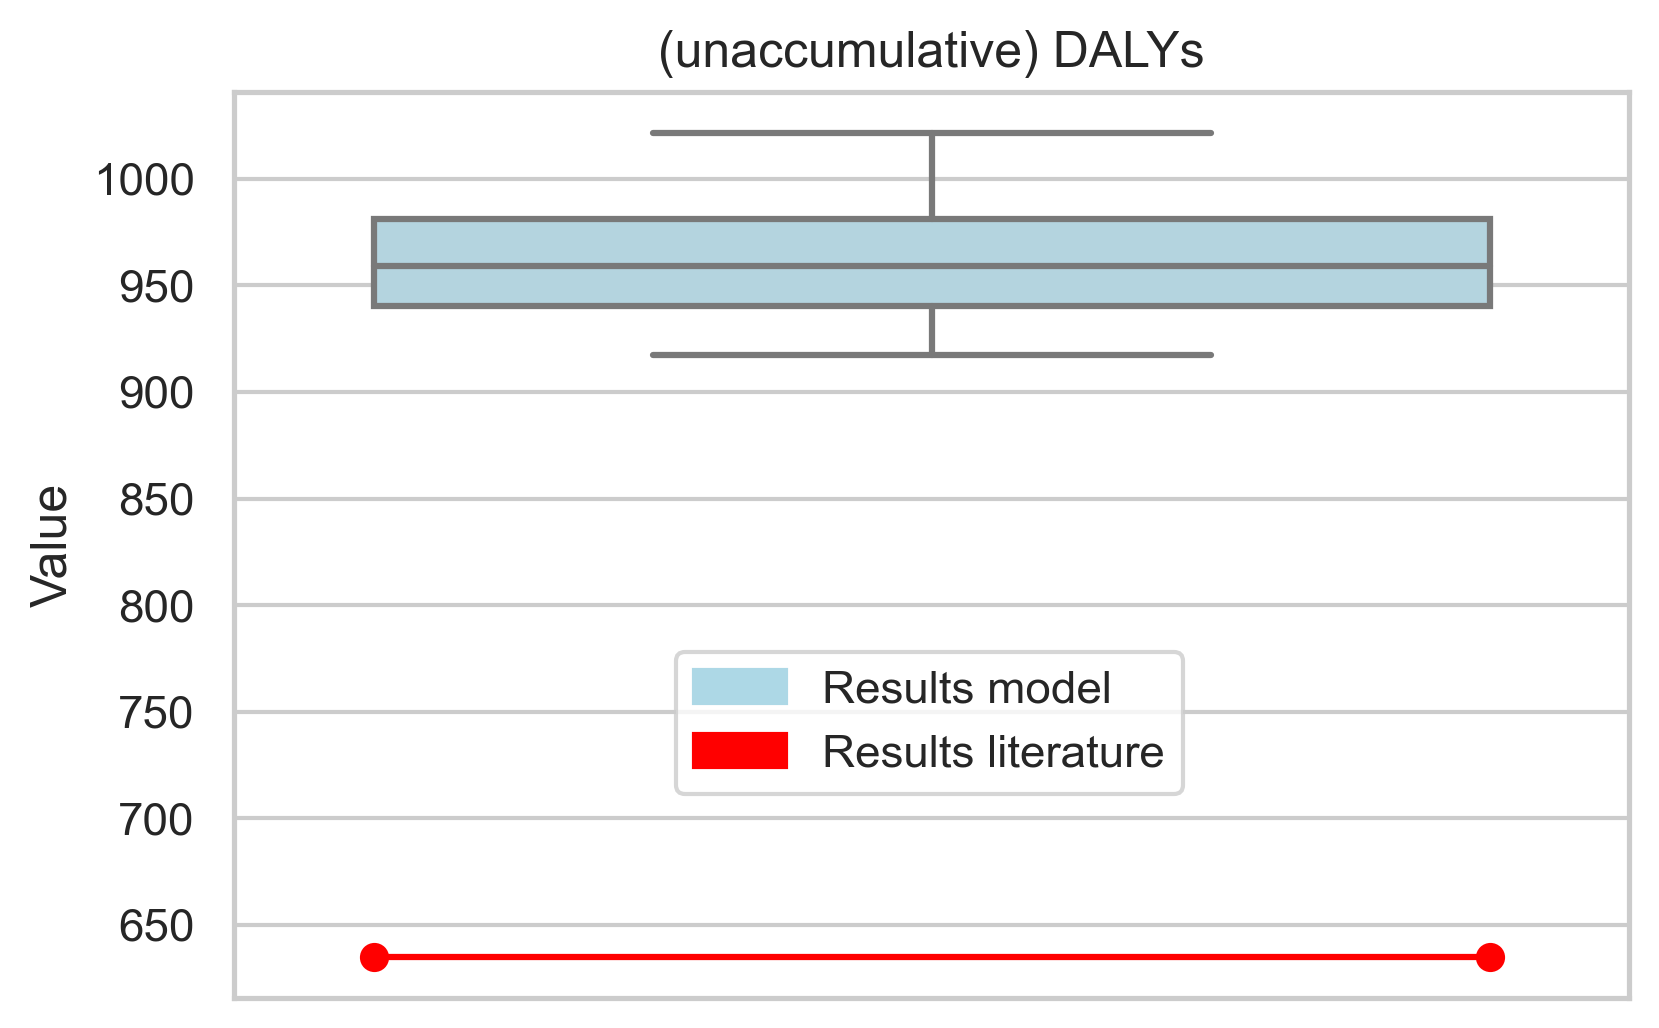
\includegraphics[width=0.9\textwidth]{notebooks/dalys2.png} % first figure itself
        \caption{Validation of DALYs}
	    \label{fig:val_dalys}
    \end{minipage}\hfill
    \begin{minipage}{0.45\textwidth}
        \centering
        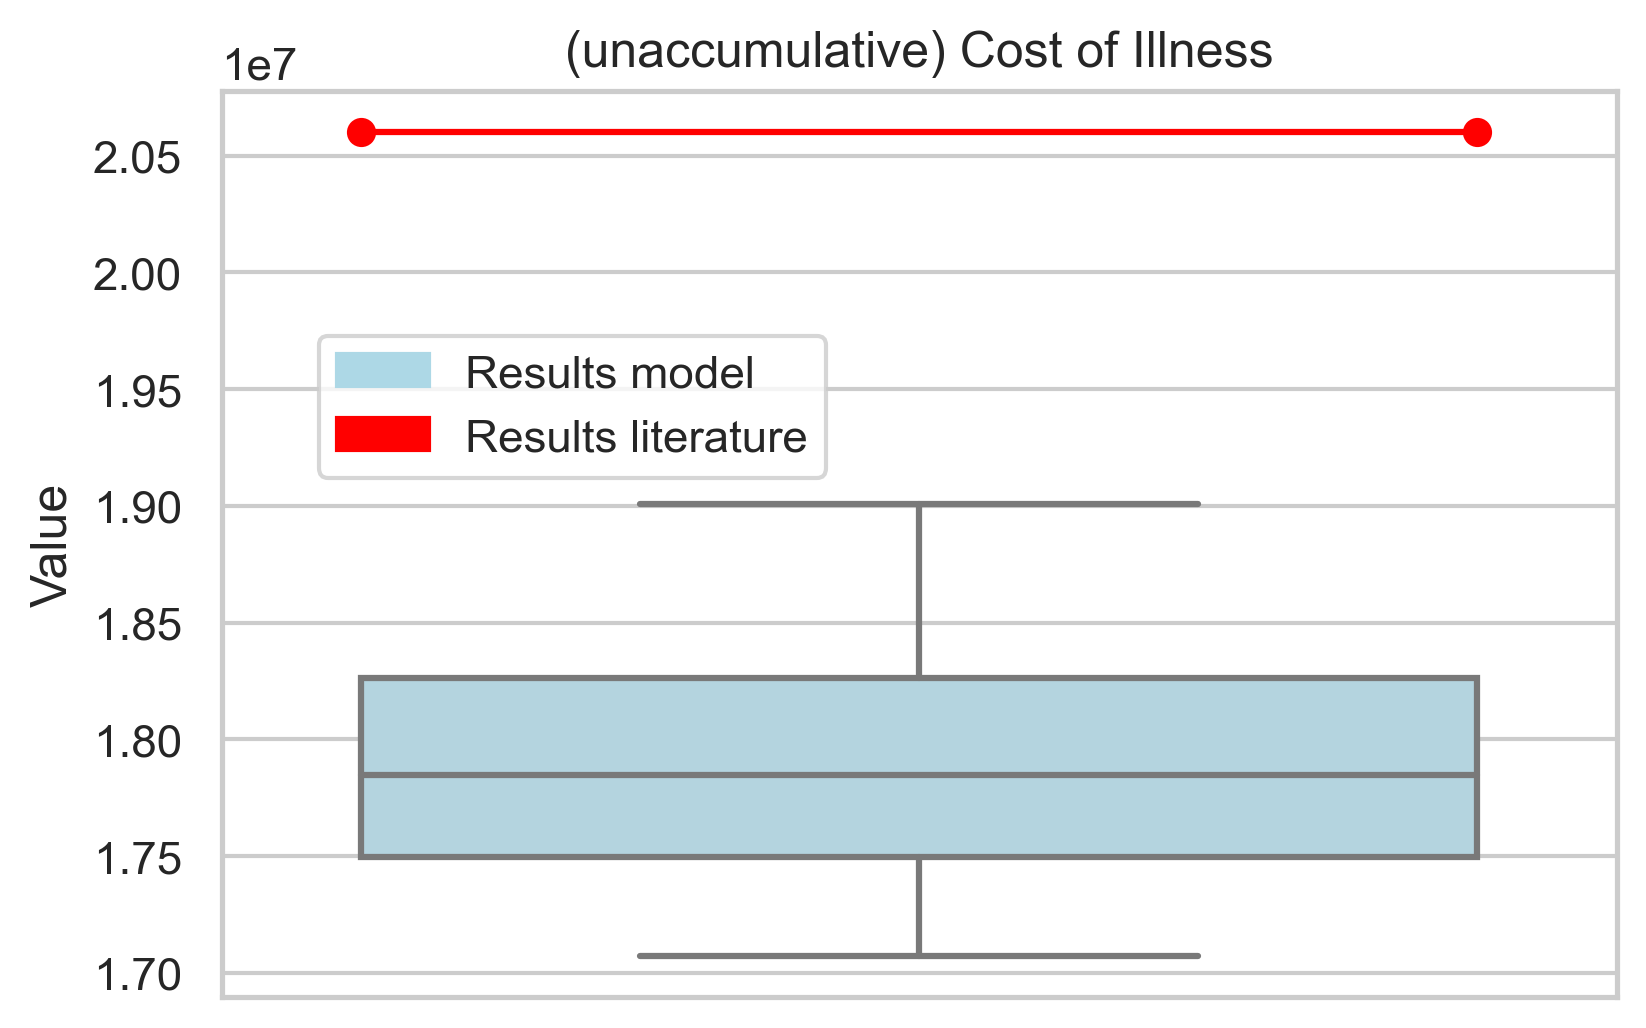
\includegraphics[width=0.9\textwidth]{notebooks/coi2.png} % second figure itself
        \caption{Validation of Cost of Illness}
	    \label{fig:val_coi}
    \end{minipage}
\end{figure*}

%TC:endignore